\Chapter{A kész játék bemutatása}

Ebben a fejezetben a játék végleges változatát fogom bemutatni, részletezve a felhasználói felületet, a játékmechanikát és a játékosok interakcióit.

A játék elindításakor a játékosok a főmenübe kerülnek. Innen a játékosok három lehetőség közül választhatnak:
\begin{itemize}
\item \textbf{Start:} "Start" gomb kiválasztásával a játékosok a szintválasztó menühöz jutnak, ahol kiválaszthatják a kívánt szintet.
\item \textbf{Options:} Ez a menü lehetővé teszi a játékosok számára az audiobeállítások módosítását, beleértve a zene és a hangeffektek hangerejét. Ezen kívül a játékosok innen érhetik el a Súgó menüt, ahol a játék mechanikáit tudják megnézni.
\item \textbf{Quit:} Ha ezt az opciót választják, a játékos kilép a játékból.
\end{itemize}

A játék menüinek és azok interakcióinak a folyamatábrája \aref{fig:menuflowchart}. ábrán megtekinthető.

\begin{figure}[ht]
\centering
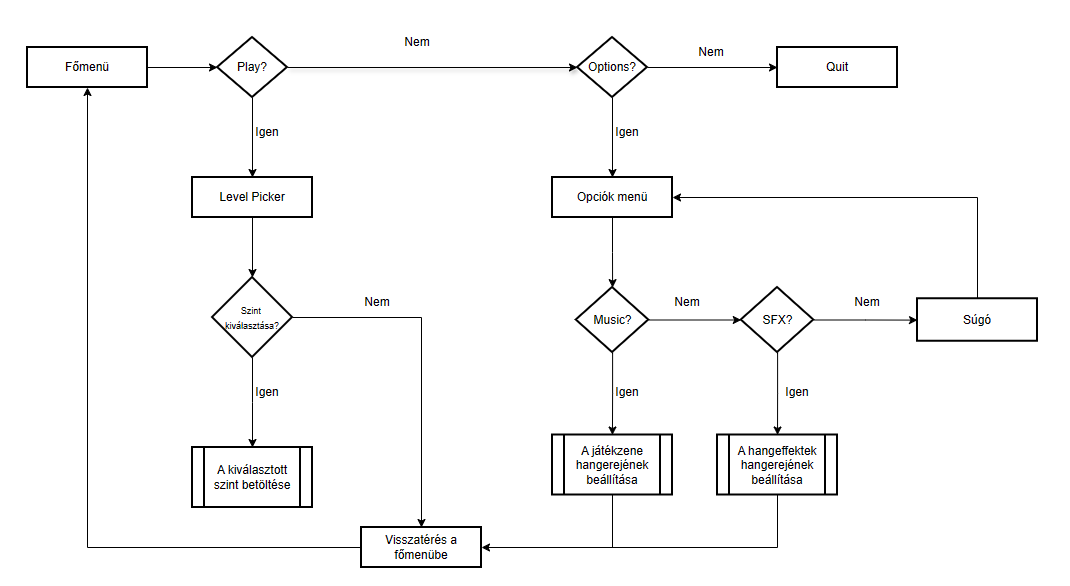
\includegraphics[width=\textwidth]{images/menuflowchart.png}
\caption{A játékban található menüknek a folyamatábrája.}
\label{fig:menuflowchart}
\end{figure}

Ha a játékos kiválaszt egy pályát, a játék betöltődik, és a játékos a pálya kezdőpontjára áll. Az összes pályán az elsődleges cél az ellenségek kikerülése, az akadályok átugrása és a rendelkezésre álló gyémántok összegyűjtése. A hátralévő gyémántok számát a képernyő bal felső sarkában lévő számláló mutatja. Egy gyémánt begyűjtése eggyel csökkenti ezt a számlálót.

A játékos az A, D, S, SPACE és SHIFT billentyűkkel tudja irányítani a főhőst. Az A billentyű lenyomásával balra, a D billentyű lenyomásával pedig jobbra tud menni a játékos. Ha a SHIFT gombot megnyomja a játékos és lenyomva tartja, akkor futni fog az irányítható karakter. A SPACE gomb gyors lenyomásával egy kis ugrást tud véghezvinni a karakter, viszont ha a játékos lenyomva tartja a SPACE billentyűt, akkor az magasabbra tud ugrani. A játékos a felvehető objektumokat az E billentyű megnyomásával tudja felvenni, a grappling hook játékmechanizmust pedig a T betűvel tudja használni. Az irányítható karakter folyamatábrája \aref{fig:playerflowchart}. ábrán megtekinthető.

\begin{figure}[ht]
\centering
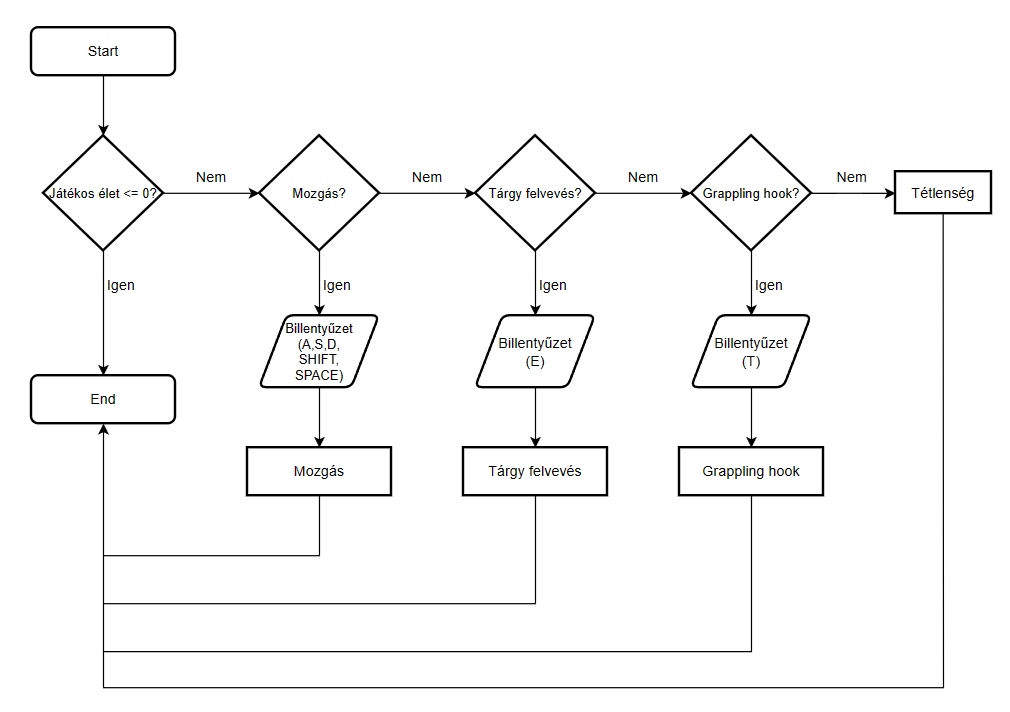
\includegraphics[width =\textwidth]{images/playerflowchart.png}
\caption{ Az irányítható karakter mozgásának a folyamatábrája}
\label{fig:playerflowchart}
\end{figure}

A játékosok minden szintet három élettel kezdenek, amelyeket piros szívek jelképeznek a képernyőn. Egy ellenséggel való találkozás egy élet elvesztését eredményezi. Az összes élet elvesztése azt eredményezi, hogy a játékos újrakezdi a szintet. Ha a játékos leesik a térképről, elveszíti mindhárom életét, és szintén újra kell kezdenie a szintet.

A játék bármikor szüneteltethető a képernyő jobb felső sarkában található szünet gomb megnyomásával. A szünet menüben a játékosoknak három lehetőségük van:
\begin{itemize}
\item A házikó megnyomásával a játékos visszatérhet a főmenübe.
\item Az elfordított háromszög megnyomásával a játékos folytathatja a játékot ott, ahol abbahagyta.
\item A minusz jel megnyomásával a játékos újrakezdheti az adott szintet.
\end{itemize}

A szünet menü \aref{fig:pausemenu}. ábrán látható.

\begin{figure}[ht]
\centering
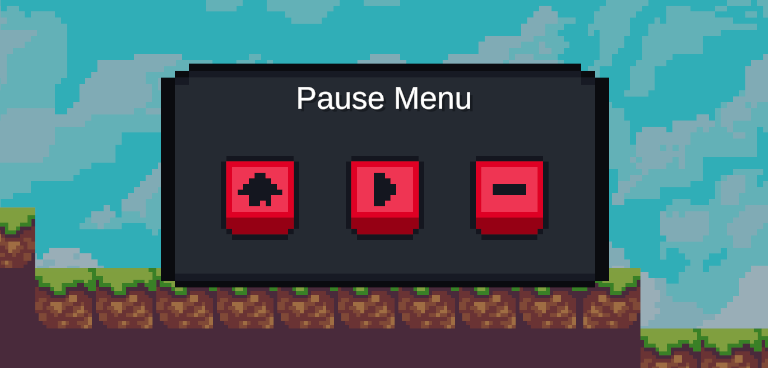
\includegraphics[scale = 0.5]{images/pausemenu.png}
\caption{A játék szünet menüje.}
\label{fig:pausemenu}
\end{figure}

Ha egy szinten belül minden gyémántot összegyűjtött a játékos, megjelenik a szint végét jelző menü, ahol a játékosok választhatnak, hogy továbblépnek-e a következő szintre, vagy visszatérnek a főmenübe. 

A szint végét jelző menü \aref{fig:finishedlevelmenu}. ábrán látható.

\begin{figure}[ht]
\centering
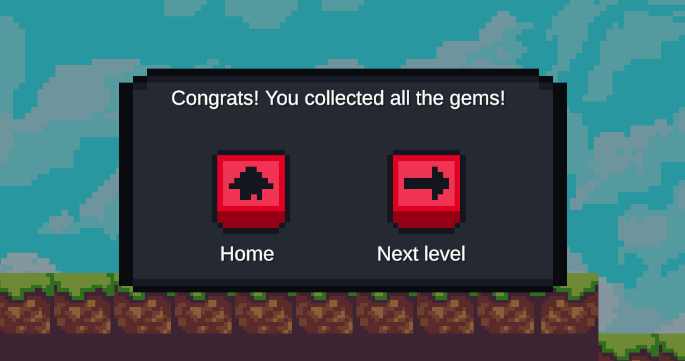
\includegraphics[scale = 0.5]{images/finishedlevelmenu.png}
\caption{Az adott szint végét jelző menü.}
\label{fig:finishedlevelmenu}
\end{figure}



